\documentclass[conference]{IEEEtran}
\usepackage[T1]{fontenc}
\usepackage{amsmath,amssymb,graphicx,booktabs,array,url}
\usepackage[hidelinks]{hyperref}
\usepackage{microtype}
\usepackage{balance}
% Repository publication is complete; the course-required video host is pending.
\newcommand{\LinkStatus}{Public source; external video hosting pending.}

% Complete current73 evidence; publication remains deferred.
\newcommand{\ResultCutoff}{Nov.\ 14, 2026, 20:47 UTC}

\newcommand{\FP}{\mathrm{FP}}
\newcommand{\TP}{\mathrm{TP}}
\newcommand{\FN}{\mathrm{FN}}
\newcommand{\R}{\mathbb{R}}
\title{Controlled VoxelNeXt Adaptation for Simulated Racing:\\Confidence, Orientation, and Closed-Loop Tradeoffs}
\author{\IEEEauthorblockN{Bradley Yong}
\IEEEauthorblockA{Blue Galaxy Racing \quad CMPE249, San Jos\'e State University\\
\footnotesize \href{https://github.com/j1s3ng/lidar-racing}{Public source repository} \quad \href{https://github.com/j1s3ng/lidar-racing/blob/main/docs/LiDAR_Racing_Demo.mp4}{112-second demo (external hosting pending)}.\\
\footnotesize Source-verified 73-case study, evidence through \ResultCutoff.\\
\footnotesize The course-required YouTube/Drive video link remains pending.}}
\begin{document}
\maketitle

\begin{abstract}
Road-trained LiDAR detectors can face different geometry and confidence distributions in autonomous racing. We study VoxelNeXt adaptation in a reproducible hybrid simulation system. Four controlled seed-7 fits use the same 10,233-cloud training pool, mining weights, initialization, and 1,200 two-cloud batches while varying trainable scope and learning rates. On 6,144 development frames, recall at raw cutoff 0.35 rises from 52.0\% for the pretrained model to 76.9\% for head-only adaptation and 95.8--96.3\% for full-network fits. A training-only cutoff rule applied to an earlier checkpoint yields 91.4\% recall and 109 false positives on 8,955 new qualification frames, versus 54.1\% and 256 for the original pipeline. At common cutoff 0.425, however, the original has only 43 false positives. Quarter-turn training improves some rotated footprints but worsens native-view recall and directed heading. An offline-qualified detector also exposes a driver halt; a fitted repair passes known hazards yet is slower in a paired 20-car engineering test. A bounded two-generation policy search improves training pace by 0.375\,s but loses 2.187\,s on paired development validation and does not advance. Five audited 60-second openers sustain 20--64 independent LiDAR streams with slower-than-wall-time physics. The reference baseline retains 127/128 clean laps and one DNF. In 30 paired confirmation cases, both policies finish clean, but the neural finalist is 3.74\% slower by paired median. Reference ranks first across four balanced 20-car heats; all 80 entries finish clean and all 24 fresh geometry cases pass. It qualifies among the four tested hybrid policies; the neural finalist is not promoted.
\end{abstract}

\section{Introduction}
Autonomous racing requires competing vehicles to be detected while relative motion, occlusion, and limited sensor returns make mistakes consequential. A road-trained detector provides a practical starting point, but adapting it is more than obtaining a successful training log: the learned weights must change, unseen capture groups must be preserved, and the deployed confidence rule must be evaluated with the model.

The original course proposal targeted fine-tuning VoxelNeXt on A2RL VMax. The dataset requires accepting access conditions~\cite{a2rlvmax}; no real A2RL training or evaluation has been completed here. We therefore report a \emph{simulation study} and retain the proposed real-data work as future work. Driving is a downstream engineering demonstration, not a replacement for the perception question or a claim of a new detection architecture.

We ask how matched scope/LR fits, confidence rules, and orientation changes affect offline and downstream behavior. Our contributions are:
\begin{itemize}
\item Matched trainable-scope and learning-rate controls, plus a separately matched TRAIN-rotation intervention with preserved native-view regressions.
\item A training-only operating-point rule, frozen before fresh pipeline qualification, with an explicit same-cutoff false-positive comparison.
\item Audited downstream failure, bounded reward-search and capacity results, with a source-bound protocol that keeps engineering evidence separate from final races.
\end{itemize}

\section{Related Work}
PointPillars encodes vertical columns~\cite{lang2019pointpillars}; CenterPoint regresses centers and attributes~\cite{yin2021centerpoint}. VoxelNeXt predicts directly from sparse voxel features~\cite{chen2023voxelnext}. We use its official implementation and nuScenes checkpoint~\cite{voxelnextcode,caesar2020nuscenes}, not a replacement backbone or a state-of-the-art benchmark claim.

Simulated vehicles, sampling and reflectance differ from both nuScenes and real A2RL racing~\cite{a2rlvmax}. Repeated synthetic track improvements cannot establish real transfer. Webots supplies physical sensors/dynamics~\cite{webots}; conventional tracking and pure-pursuit-style actuation~\cite{coulter1992pursuit} complement the neural policy.

The resulting driver combines supervised distillation with bounded derivative-free, reward-based output calibration using the cross-entropy method (CEM)~\cite{rubinstein1999cem,deboer2005cem}. Its conventional guard and controller remain active. RGB is recorded for visualization and is not a policy input; neither the detector nor driver is an end-to-end camera model or policy-gradient system.

\section{Methodology}
\subsection{System and information boundaries}
Figure~\ref{fig:architecture} shows the deployed data flow. Each moving car receives its own LiDAR point cloud and sends only measured point features to a CUDA service. The response contains predicted boxes, confidence scores, and timing metadata. Geometric raw-LiDAR hazards complement semantic car detections. A 48-feature neural policy produces speed and lane decisions; a conventional guard and actuator controller execute those decisions in vehicle physics.

Own localization and a reference map are available to the driver. Opponent supervisor poses are used for offline labels and independent evaluation only. Runtime source inspection, recorded assertions, and separate trace/evaluator joins check this boundary. The system does not infer ego localization from the LiDAR detector, and the experiments do not evaluate a complete autonomous localization stack.


\begin{figure*}[t]
\centering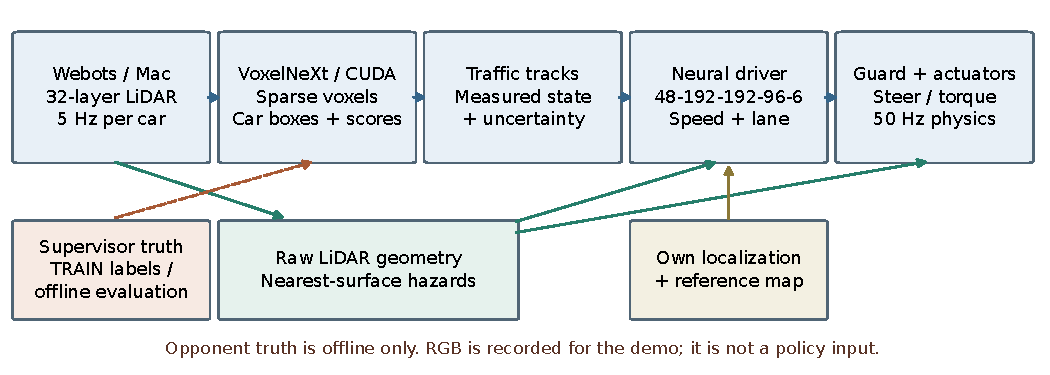
\includegraphics[width=7in]{figures/architecture.pdf}
\caption{Implemented data flow. Solid arrows carry measured sensor/model/control data. The separate supervisor channel provides labels and offline scoring. The dashed truth arrow denotes offline detector supervision only. Own pose/map remain available; RGB is recorded but is not a model input.}
\label{fig:architecture}
\end{figure*}

\subsection{Simulated data and split discipline}
The world approximates a 5,227.13\,m Yas Marina lap using public position data and a generic Webots vehicle. It is not a surveyed circuit, an exact F1 racing line, or a calibrated F1 tire model. The vehicle mass is 880\,kg and the configured friction coefficient is 1.5. Physics runs at 20\,ms, with LiDAR/camera sampling at 200\,ms. The LiDAR has 32 layers, 1,024 horizontal samples, and a 100\,m maximum range. Detection scoring uses a separate 50\,m XY region.

Training exports contain 10,233 clouds and 16,613 visible car targets. The moving development capture contains 6,144 deduplicated clouds and 8,155 targets. Within each experiment, all car viewpoints from a capture share one role; source-config identities and exact cloud hashes are checked for overlap. Qualification, confirmation, and championship sources are excluded from fitting by default, including ancestor-directory seals and resolved symbolic-link paths. Historical data-role releases are explicit and recorded; they do not silently reclassify later qualification captures.

New captures still share the simulated vehicle and track. Capture-level separation reduces direct leakage, but does not make frames independent or establish geographic or real-world generalization. We do not treat thousands of correlated frames as thousands of independent trials.

\subsection{Detector and actual fine-tuning}
For a measured cloud $P=\{(x_i,y_i,z_i,r_i)\}_{i=1}^{N}$, the input adds a zero time-lag feature and uses the official voxel encoder. Webots provides geometric returns; intensity $r_i$ is a constant 1.0 placeholder, not physical reflectance. The original ten-class architecture is preserved, while evaluation retains the car class. The configured voxel sizes are $(0.075,0.075,0.2)$\,m. The single-frame simulation input differs from the original multi-sweep pretraining distribution; no simulated temporal sweep accumulation is claimed.

The historical full-network pilot starts from the official checkpoint and performs 1,200 AdamW updates, batch size two, weight decay $10^{-4}$, gradient clipping at norm 10, backbone LR $10^{-5}$, and head LR $10^{-4}$. Batch-normalization running statistics are fixed. Official detection losses are retained with localization weight 0.25, while the two velocity-code weights are zero because this study does not supervise the pretrained velocity task. For a batch $B$, the implemented objective is
\begin{equation}
\mathcal{L}(B)=w(B)\left[\mathcal{L}_{\rm cls}(B)+0.25\mathcal{L}_{\rm loc}(B)\right].
\end{equation}
Here $w(B)=3$ for a batch without targets and $w(B)=1$ otherwise. Half the batches are homogeneous negative batches. Scene-balanced sampling and training-only hard-negative mining emphasize empty-frame errors. The historical pilot and four controlled base arms use no geometric augmentation or database pasting; the separately matched fifth fit adds TRAIN-only quarter turns. The selected hard-negative pool contains 576 training frames; development or qualification data are not mined.

The 2,400 draws use replacement (1,398 distinct IDs), rather than a complete training-pool pass; all clouds remain available for mining/calibration. Strict reload checks all 542 state tensors. Full-model first-step audits verify 121 nonzero finite backbone gradients and an actual saved convolution update. Historical timing fields include optimizer setup, fitting and adapted evaluation, not pure optimizer throughput. The historical qualified artifact remains distinct from later controlled fits; development gains do not confer qualification.

\subsection{Training-only pipeline calibration}
Raw score 0.35 is the original deployment cutoff. After the fixed-0.35 adapted artifact fails fresh false-positive gates, we preserve those outcomes and declare a genuinely different confidence pipeline. For $\tau\in\{0.35,0.375,\ldots,0.95\}$, the rule is
\begin{equation}
\begin{aligned}
\tau^*&=\underset{\tau}{\arg\max}\;R_{\rm train}(\tau)\\
\text{s.t.}\quad&\FP_{\rm train}(\tau)/F_{\rm train}\leq0.01,\\
&R_{\rm train}(\tau)\geq R^{\rm original}_{\rm train}(0.35).
\end{aligned}
\end{equation}
Ties choose the lower cutoff. This selects 0.425: training FP falls from 219 to 101 (0.00987/frame), with recall 0.9208 versus the original training recall 0.5293. Lower grid cutoffs violate the 0.01 budget . The learned tensors are unchanged by calibration.

The new artifact binds its effective cutoff, configuration, calibration rule, source hashes, and qualification reservation. It is frozen before scoring two new reserved capture groups. This is a new pipeline qualification, not a rerun of the rejected artifact under a loosened gate. Original and adapted deployment cutoffs differ in the successful comparison; the result cannot be attributed to learned weights alone.




\subsection{Driving and physical verification}
The learned driver is a supervised $48\!\rightarrow\!192\!\rightarrow\!192\!\rightarrow\!96\!\rightarrow\!6$ ReLU MLP: three per-lane speed values and three lane logits. It distills measured-hazard trajectory costs, supplemented by eligible reference-drive examples. It uses measured tracks and raw geometric hazard summaries, including propagated position and velocity uncertainty. Measurement age affects upstream tracking/covariance rather than being a separate neural input. A predictive guard checks the proposed motion and can reduce speed or restrict lane motion. Steering and wheel actuation remain conventional. Thus a clean race tests the combined system, not the neural network in isolation.

The Rich005 training revision adds realistic fresh/aged track examples and teaches stable passing intent: an emerging side choice is retained only when alternatives have similar costs and the same collision status; a clearly blocked side overrides that preference. Evaluation compares frozen driver checkpoints with unchanged runtime code, guard, world, and detector. Because training data and teacher supervision change together, this is a controlled \emph{system revision comparison}, not an isolated causal ablation of the intent term.

Each attempt records source, checkpoint, detector, rule, and scenario hashes. Scoring requires authored control/results files and a fresh independent audit. A clean finish requires the complete lap plus zero scored vehicle-envelope overlaps, track violations, and pose resets after spawn. Staggered runoff parking keeps finished cars from blocking active cars. These conservative sampled-envelope checks are not a real-vehicle safety guarantee.

\subsection{Bounded reward-based policy search}
CEM searches affine output calibrations of the supervised Rich005 seed-17 driver. Its budget is two generations of six proposals. Each proposal receives four engineering hazard cases, followed by a four-car race only if all four pass. Complete clean finishes determine feasibility before a mean-pace reward with a 480\,s cutoff. Up to two highest-reward feasible proposals update the sampling distribution. Speed gain is bounded to $[0.92,1.08]$, speed offset to $[-1,1]$\,m/s, and three zero-mean lane-logit biases to $[-0.2,0.2]$. The calibrations are folded into exported output weights/biases. A nonidentity proposal must improve by at least 1\,s in paired seed-211 development validation before eight- and twenty-car engineering eligibility checks. Formal confirmation or championship outcomes never guide this search or finalist selection.

\section{Experiments and Comparisons}
\subsection{Hardware and metrics}
An Apple M4 Max Mac (128\,GB unified memory) runs Webots. The LAN host provides an RTX PRO 6000 Blackwell workstation GPU and an RTX 3090. The recorded fine-tune uses PyTorch 2.13.0+cu130 and CUDA 13.0. Runtime manifests preserve exact software/source identities rather than assuming a package name uniquely identifies an environment.

Detection metrics use car targets with at least three measured points, within 50\,m XY range. Score-ordered greedy matching assigns each prediction to its nearest unmatched target within 2\,m XY center distance. With $F$ frames,
\begin{equation}
R=\frac{\TP}{\TP+\FN},\qquad \FP/F=\frac{\#\text{unmatched predictions}}{F}.
\end{equation}
These are custom center-distance diagnostics, \emph{not} official nuScenes/A2RL AP or 3D-IoU AP. Center-error comparisons on the common matched-object subset reduce selection differences, but still condition on successful matching; recall is reported alongside them. Far-range recall uses targets at 30--50\,m XY range, with an additional gate when at least 30 such targets are present. Directed heading distinguishes front/back; a separate $\pi$-symmetric box heading does not. BEV IoU measures the planar footprint. No official heading/AP benchmark is claimed.

\subsection{Matched scope and learning-rate controls}
Four new seed-7 fits start from the same original checkpoint and use the same frozen data, batch size two, 1,200 steps, initialization, miner, and evaluation. The arms are head-only LR $10^{-4}$; full-network uniform LR $10^{-4}$; full-network uniform LR $10^{-5}$; and full-network mixed head/backbone LR $10^{-4}/10^{-5}$. All 1,200 actual batches, 2,400 frame draws, mining identities and sampling weights match. Small floating-point differences in raw miner scores are preserved without changing the resulting weights. Head-only changes zero backbone tensors, while every full arm changes all 121 audited backbone tensors; all 204 BN running buffers remain fixed. The architecture has 7,981,398 scalar parameters, of which 612,678 are optimized head-only. Trainable scope does not change inference architecture size.

Figure~\ref{fig:controlled} reports the same 6,144 DEV frames and 8,155 targets at RAW .35. Original recall/FP is 51.98\%/96; head-only reaches 76.87\%/33. Full uniform $10^{-4}$, uniform $10^{-5}$, and mixed reach 95.77\%/51, 96.27\%/75, and 95.76\%/81. No arm dominates every measure. On the fixed 3,953 targets matched by all five models, XY center error is .283\,m for original and .237/.110/.180/.166\,m for the four fits. This conditional intersection excludes misses, so all-target recall remains necessary. These single-seed development controls supersede earlier unmatched head/full comparisons, but do not identify a universally best learning rate or inherit historical pipeline qualification.

\begin{table}[t]
\caption{Score-swept BEV AP on known simulated DEV data.}
\label{tab:bev-ap}
\centering\small\setlength{\tabcolsep}{3pt}
\begin{tabular}{lr}
\toprule
Detector & BEV AP@0.5 (\%)\\
\midrule
Original & 81.557\\
Head-only $10^{-4}$ & 88.471\\
Full uniform $10^{-4}$ & 96.838\\
Full uniform $10^{-5}$ & 97.671\\
Full mixed & 94.995\\
Full mixed + quarter turns & 94.652\\
\bottomrule
\end{tabular}
\end{table}

On the same 6,144 known DEV frames (8,155 eligible cars), Table~\ref{tab:bev-ap} reports global score-ranked, one-to-one BEV IoU matching at 0.5 and 101-point interpolated AP. All models use NMS IoU 0.2, post-NMS cap 83 and cached score floor 0.1; unmatched predictions with BEV IoU at least 0.5 to excluded ground truth are ignored. This score sweep is distinct from recall at cutoff 0.35. It is fixed-postprocessing simulated DEV evidence, not an official benchmark or an independent test.

\begin{figure*}[t]
\centering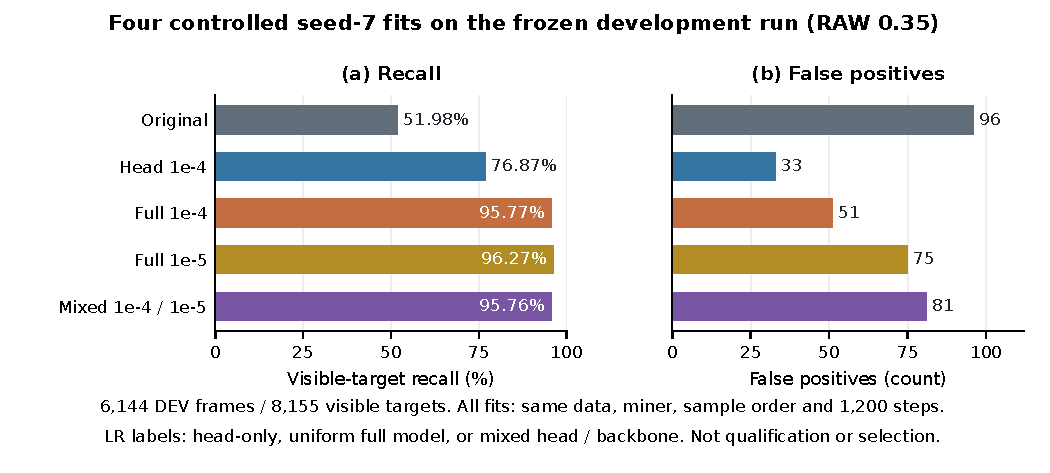
\includegraphics[width=7in]{figures/controlled_ablation_compact.pdf}
\caption{Four actual matched seed-7 fits at common RAW .35. Scope/LR differ; original initialization, data, miner weights, sample order, 1,200 updates, and evaluation match. This is development evidence, not fresh qualification or checkpoint selection.}
\label{fig:controlled}
\end{figure*}

\subsection{Matched TRAIN rotation: native-view negative}
A separate fifth fit repeats mixed-rate seed 7 with the exact same mining/sample sequence. An independent RNG applies $0,90,-90,180$ degree turns only to TRAIN items, consistently transforming points, GT centers, yaw and XY velocity labels while preserving Z/intensity/time lag. Mining/evaluation remain unrotated. All 2,400 angle draws and inverse/alignment audits are recorded; maximum box-corner error is below $3.2\times10^{-7}$\,m. Actual nonzero gradients and saved-backbone changes confirm a fitted intervention.

The same unrotated 6,144-frame cache shows a negative result at both cutoffs (Table~\ref{tab:augmentation}). At .35, paired center error worsens .171 to .192\,m on 7,671 common targets; directed yaw rises .111 to .621\,rad (6.36 to 35.58 degrees). At .425, the intersection is 7,431 and yaw rises .109 to .615\,rad. Slight improvement in $\pi$-symmetric box heading does not remove the front/back error. No qualification, deployment, or threshold selection follows from this analysis.

\begin{table}[t]
\caption{Matched mixed/Aug pair: same 6,144 native-view DEV frames, 8,155 targets. Filtering saved caches upward performs no new model query.}
\label{tab:augmentation}
\centering\small\setlength{\tabcolsep}{4pt}
\begin{tabular}{lrrrr}
\toprule
Raw cutoff & Mixed R & Aug. R & Mixed FP & Aug. FP\\
\midrule
.35 & 95.76\% & 94.67\% & 81 & 105\\
.425 & 93.78\% & 92.00\% & 34 & 50\\
\bottomrule
\end{tabular}
\end{table}

\subsection{Known DEV rotation stress diagnostic}
We score 128 already inspected DEV clouds under four rigid rotations. Recall uses all 174 visible targets per angle; geometry uses the same 41-target all-model/all-angle intersection. Quarter-turn training improves rotated footprint IoU yet worsens native-view directed yaw. These correlated, design-informed DEV views are diagnostic, not fresh scene qualification or model selection.

\begin{figure*}[t]
\centering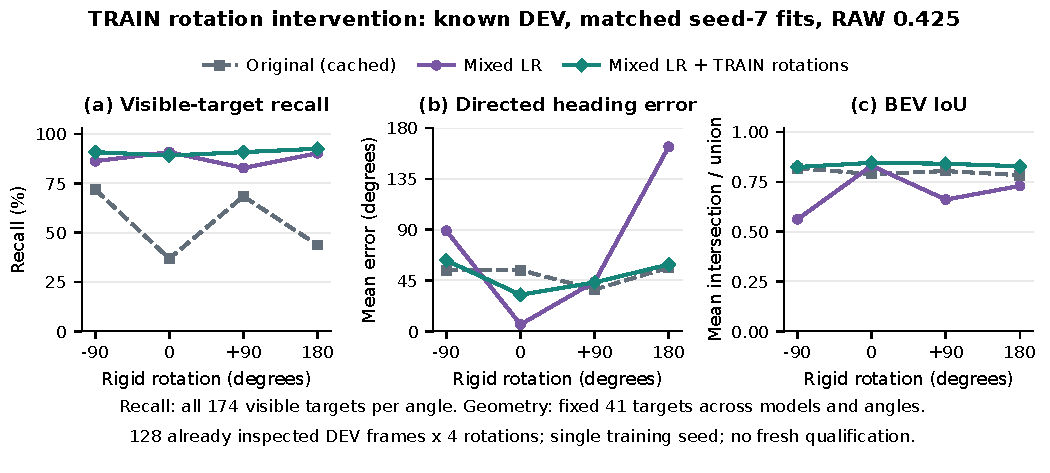
\includegraphics[width=7in]{figures/rotation_compact.pdf}
\caption{Known DEV sensitivity at RAW .425, one matched training seed. Recall: 174 targets/angle. Geometry: fixed 41-target all-angle intersection. Original predictions are cached. TRAIN rotation improves rotated footprints but worsens native directed heading. Native seven-inch vectors retain text at least 8.2\,pt.}
\label{fig:rotation}
\end{figure*}

\subsection{Historical fixed-cutoff adaptation and failed qualification}
For the historical pilot at raw cutoff 0.35 for both models, moving-development recall increases from 52.0\% to 95.7\%, while FP falls from 96 to 79 over 6,144 clouds. Mean center error on common matches decreases from 0.293 to 0.171\,m. This is promising development evidence but does not imply unseen-group qualification.

Two subsequent groups expose the failure (Table~\ref{tab:detector}). Adapted recall remains high, but FP/frame reaches 0.0421 and 0.0374, exceeding the predeclared absolute cap of 0.02 on both groups. The failures are retained. Earlier head-only pilots also failed subsequent FP checks: a 600-step model produces 65 FP over 2,540 frames (0.0256/frame) on its reserved capacity capture. Different budgets, data, and capture groups prevent interpreting these exploratory pilots as a fair head-only versus full-network benchmark.

A recorded development illustration adds an unmatched score-.364 box while recovering three missed cars. It is a chosen failure example, not a representative qualification sample or an experiment selecting a cutoff.

\begin{table*}[t]
\caption{Detector results by capture group. Baseline cutoff is 0.35 throughout. ``Old'' and ``new'' qualification groups are different captures; cross-row comparisons do not isolate calibration. Recall and FP/frame are evaluated within each row.}
\label{tab:detector}
\centering\small\setlength{\tabcolsep}{4pt}
\begin{tabular}{lrrrrrrl}
\toprule
Role / group & Frames & Cutoff & Base R & Adapt R & Base FP/F & Adapt FP/F & FP cap\\
\midrule
Development: moving & 6,144 & .35 & 52.0\% & 95.7\% & .0156 & .0129 & --\\
Old: clean20 & 1,474 & .35 & 55.3\% & 92.7\% & .0427 & .0421 & Fail\\
Old: seed79 & 4,040 & .35 & 50.9\% & 93.3\% & .0344 & .0374 & Fail\\
New: mixed20 & 6,040 & .425 & 54.5\% & 91.8\% & .0298 & .0136 & Pass\\
New: reference20 & 2,915 & .425 & 53.0\% & 90.4\% & .0261 & .0093 & Pass\\
New: aggregate & 8,955 & .425 & 54.1\% & 91.4\% & .0286 & .0122 & Both pass\\
\bottomrule
\end{tabular}
\end{table*}

\subsection{New calibrated-pipeline qualification}
On 8,955 new qualification frames with 20,536 visible targets, aggregate recall increases from 0.5407 to 0.9139. FP decreases from 256 to 109, or 0.0286 to 0.0122/frame. Each group separately satisfies six predeclared gates: recall nonregression; FP/frame at most 0.02 and increase at most 0.01; common-match center error at most 0.5\,m and degradation at most 0.1\,m; and far-range recall nonregression. Per-group common-match center errors improve from 0.303/0.295 to 0.168/0.175\,m; aggregate far recall increases from 0.548 to 0.845. The exact per-group gate definitions and decision records accompany the report.

The successful comparison changes weights \emph{and} cutoff. It qualifies this historical detector pipeline for physical trials, not a later controlled fit or an automatically promoted driving system. Capture groups remain correlated within the same synthetic domain; frame-level confidence intervals would overstate independence.

\subsection{Post hoc confidence ablations}
We additionally reuse the closed prediction caches at a common raw cutoff of 0.425, already selected from training data before qualification. Stored scores are unchanged model confidences, not remapped calibrated probabilities. The original cache retains predictions down to 0.1; the adapted cache is truncated at 0.425. Filtering both upward to 0.425 is therefore valid, whereas reconstructing adapted 0.35 performance on these new captures is impossible from this cache. The original matching function and frozen visible-target records are reused without inference, fitting, or a qualification-decision rewrite.

Table~\ref{tab:cutoff} isolates two effects. For the original model alone, increasing the cutoff reduces recall from 54.1\% to 39.6\% and FP from 256 to 43. At the common 0.425 cutoff, adaptation increases recall to 91.4\% but also increases FP to 109. Common-match center error improves from 0.293 to 0.167\,m on 8,107 common targets, and far recall from 0.382 to 0.845. Thus the recall/localization benefit persists at equal cutoff, while the earlier FP-reduction statement applies specifically to the deployed 0.35-versus-0.425 pipeline comparison. Equal raw confidence is not a matched-precision operating point.

\begin{table}[t]
\caption{Post hoc confidence ablation on the same 8,955 new qualification frames. The frozen original qualification decision is unchanged.}
\label{tab:cutoff}
\centering\small\setlength{\tabcolsep}{4pt}
\begin{tabular}{lrrrr}
\toprule
Weights & Raw cutoff & Recall & FP & FP/frame\\
\midrule
Original & .35 & 54.1\% & 256 & .02859\\
Original & .425 & 39.6\% & 43 & .00480\\
Adapted & .425 & 91.4\% & 109 & .01217\\
\bottomrule
\end{tabular}
\end{table}

A retrospective same-tensor cutoff change on the old 5,514-frame cohort reduces FP from 213 to 102 and recall .9318 to .9101. It neither turns the rejected artifact into a fresh pass nor selects a new threshold.

\subsection{Driver revision and multi-car demonstration}
With the original detector, Rich005 seed 17 passes four known stopped-car engineering scenarios and completes clean 4-, 8-, and 20-car fields. The 20-car field finishes in 237.787--307.448\,s (mean 280.069\,s). Its independent audit joins 30,860 own-pose samples exactly to the evaluator and checks physical finish crossings. This supports a working multi-car demonstration, not a universally best AI racer.

A later Rich006 revision passes all four audited known calibrated-perception hazards, including the previously failing left-blocked case and completes a separate homogeneous 20-car engineering field with 20/20 clean full laps. Its fitted/design-informed cases do not establish untouched-layout generalization. A hazard starting at ordered progress 2,900\,m and crossing 5,227\,m is only a partial route; the separately audited field supplies the full-lap evidence.

With original perception, Rich005 seed 17 and Rich006 seed 17 both finish 20/20 clean in a paired engineering comparison: same seed 83, 14\,m spacing, .3\,m jitter, 70\,m horizon, reference, rules, spawn identities, and all eight runtime hashes. Both actually use 12 PRO streams plus eight RTX 3090 streams. Mean times are 280.069 and 283.219\,s, respectively: Rich006 is 3.150\,s slower and faster in only 5/20 corresponding grid slots. Training/teacher revisions are combined, not a single-feature ablation. Logging stride and background workload differ, so wall-time ratios are not causal driver/GPU benchmarks. The calibrated-perception Rich006 field has different GPU placement and is not another driver-only comparison.

The verified 116-second movie presents 8\,s of context, 100\,s retaining every frame of the first heat's 311-second source, and 8\,s of results. LiDAR and predictions join the exact car/frame/capture time, with sample age shown. Standings are visualization only. Normal-speed footage and onboards are retained. The first-heat winner, Rich005 seed 7, differs from the aggregate winner.

\subsection{Bounded search: training gain fails development validation}
Both CEM generations complete six proposals. All 12 pass their four hazards and conditional four-car race: 48 hazard cases and 12 fitness races, followed by two paired validation races. The best training proposal lowers mean pace from 246.514 to 246.139\,s, a 0.375\,s improvement. On the separate seed-211 development pair, the identity calibration takes 245.828\,s and the proposal 248.014\,s. Both are clean, but the improvement is $-2.187$\,s, below the required $+1$\,s. The searched proposal therefore does not advance to larger-field eligibility or formal evaluation. This negative result prevents a small training reward gain from being called a better racer.

\subsection{Measured capacity and runtime scope}
Table~\ref{tab:capacity} replaces early unmatched opening trials with five matched 60\,s simulated openers. Each car supplies 300 distinct 5\,Hz sensor frames, yielding 56,400 verified cloud/prediction/action joins. All five opening windows are clean and have zero client inference failures. Streams are split equally between PRO 6000 and RTX 3090, from $10+10$ to $32+32$; the calibrated service remains resident but unused. Physics uses eight threads with the same frozen reference driver, original detector, seed, spacing and capture settings.

\begin{table}[t]
\caption{Audited 60\,s openers, 300 sensor frames per car. RTF is simulated time/director wall time; RPC includes serialization, network, queuing and model work. No full lap is claimed at 24--64 cars.}
\label{tab:capacity}
\centering\small\setlength{\tabcolsep}{4pt}
\begin{tabular}{rrrrr}
\toprule
Cars & Frames & RTF & RPC p95, ms & RPC p99, ms\\
\midrule
20 & 6,000 & .637 & 210.9 & 217.7\\
24 & 7,200 & .543 & 242.1 & 249.8\\
32 & 9,600 & .413 & 310.7 & 319.7\\
48 & 14,400 & .265 & 430.9 & 448.9\\
64 & 19,200 & .196 & 551.8 & 584.3\\
\bottomrule
\end{tabular}
\end{table}

The 64-car opener sustains all 64 streams through 60 simulated seconds, taking 306.7\,s of director wall time. The 5\,Hz rate is per simulated second, not wall second. This is a measured operating point, not a global capacity maximum or 64-car full lap. The 20/24/32 trials overlap independent CPU tests/audits; deep analysis is deferred during 48/64. GPU telemetry is absent for 20/24, covers two late samples for 32, and partial polling windows for 48/64. Sampled maxima cannot establish total device peaks or headroom. Startup/preflight/teardown belongs to separate queue wall time; neither interval isolates startup alone.

The four matched fits each take about 481--518\,s through loading, mining, fitting and adapted evaluation; augmentation takes 517.8\,s. These are not optimizer-only timings. The known-rotation executor completes 2,560 scored forwards and ten warmups in 68.6\,s with resident services. Host timing includes CPU preparation, transfer, model and NMS. PyTorch allocated peaks exclude context, custom spconv and other non-PyTorch memory. Neither is an isolated hardware benchmark; no T4 is measured.

\subsection{Complete final evaluation and qualified ranking}
All 73 required cases are independently source verified: the original 15-case reference baseline, 30 paired confirmations, four balanced heats, and 24 fresh geometry cases. The baseline retains 127/128 clean laps and one 20-car DNF. Valid-lap means are 242.747/249.438/263.346\,s for 4/8/20-car strata; the last excludes the DNF.

On fresh confirmation, reference and the engineering-frozen Rich005 seed-7 finalist each achieve 128/128 clean laps and 3/3 hazards. Their 4/8/20-car mean times are 242.352/249.238/264.365\,s and 246.894/255.896/277.416\,s, respectively. Across 128 corresponding clean pairs, the median neural/reference time ratio is 1.03737. The neural policy is 3.74\% slower and lacks the required strict improvement, so no promotion occurs; Reference remains incumbent.

In four mixed-policy 20-car heats, every policy occupies each grid position exactly once. All 80 entries finish valid and clean, and each policy wins one heat. All four winners start at grid index 1, limiting causal interpretation of heat wins. Ranking first compares clean completion and completion rates, then mean position and mean valid time. Reference therefore qualifies among these four tested policies (Table~\ref{tab:final}); this is not a global best-policy claim. Rich005 seed 17 supplies the fastest individual finish, 236.124\,s in heat 2, which does not determine the aggregate rank. All four policies pass their six separately audited fresh geometry cases (24/24).
\begin{table}[t]
\caption{Four balanced 20-car heats: each policy has 20 starts, one at every grid position, and one heat win. All finish clean; mean position then determines rank. Reference passes its six fresh geometry cases and qualifies among these policies.}
\label{tab:final}
\centering\small\setlength{\tabcolsep}{4pt}
\begin{tabular}{lrrr}
\toprule
Policy & Clean & Mean position & Mean lap, s\\
\midrule
Reference & 20/20 & 8.75 & 268.808\\
Rich005 seed 17 & 20/20 & 9.70 & 273.441\\
Rich006 seed 17 & 20/20 & 11.75 & 280.401\\
Rich005 seed 7 & 20/20 & 11.80 & 280.027\\
\bottomrule
\end{tabular}
\end{table}


\section{Failure Analysis and Limitations}
\subsection{False positives and unsupported filtering hypotheses}
The rejected fixed-0.35 model's 213 false positives on the old qualification groups comprise 145 background detections, 43 centers displaced 2--4\,m, 19 boundary cases, five sparse-target exclusions, and one duplicate under the saved taxonomy. Boundary errors are a minority, so merely trimming the scoring ROI would not address the dominant failure and would change the evaluation question. Six candidate point-support filters also fail to retain sparse/side recall while satisfying the FP requirements. These negative results motivate calibrated confidence rather than an unverified geometric fix. Calibration still does not solve synthetic-domain bias.


\subsection{Offline detection gains do not validate the driver}
A matched single-pair experiment replaces only the detector pipeline while keeping the Rich005 checkpoint, all eight runtime source hashes, rules, reference, seed, configured starts, and observed initial physical poses identical. The original pipeline passes the 3,000\,m stopped-car case; the new calibrated pipeline halts at progress 2,990.006\,m, short of the required 3,020\,m. Both attempts are fully audited with zero scored incidents. This is a valid halt failure, not missing infrastructure evidence.

Requested speed first diverges at 6.2\,s, and the new-pipeline trajectory chooses the blocked left side at 7.2\,s while the original trajectory stays right. A frozen-state intervention is diagnostic: removing semantic detection rows alone leaves the wrong left decision; removing one aged geometric fragment with positional uncertainty 9.125\,m changes the prediction to the teacher's right side with probability 0.969. This suggests a driver sensitivity to aged raw-feature aliasing exposed by the changed trajectory. It is a \emph{one-state ablation and causal hypothesis}, not proof that semantic false positives caused the halt, an on-policy repaired result, or a general detector ranking. The fitted Rich006 revision subsequently passes the known engineering gates, including that previously failing left-blocked case, as reported above; that is a separate on-policy known-case result, not fresh generalization or proof of the one-state causal hypothesis.

\subsection{Infrastructure failures are not policy rewards}
Session-bound detector/tunnel exits leave 60 early attempts without authored results or initialized sensors. Attempted 24/32-car cases in that incident provide no capacity evidence. A later synchronous mid-run disconnect is separately preserved as interrupted infrastructure evidence, not a policy failure or completed lap.

Recovery uses detached service/tunnel supervisors, finite restart/deadline leases, exact process identities and measured-cloud readiness. New suites/search IDs preserve invalid history. Evaluation reservations release the exact queue only after owned CPU/GPU workers exit and three real service checks pass. No held-out or tournament win is inferred from engineering recovery.

\subsection{Scope and remaining evidence}
Only one matched training seed is evaluated. Controlled scope/LR and quarter-turn augmentation comparisons are now complete on the declared development inputs; a second seed, real A2RL benchmark AP, isolated latency/memory profiling, a T4 comparison, and live ROS2 replay remain incomplete. Repeated geometry, simplified reflectance, a generic vehicle/tire model, trusted own pose/map, and hybrid control limit deployment claims. Directed front/back errors can coexist with good symmetric footprint estimates. Passing offline gates does not imply real-world safety. The complete protocol supports Reference among four tested policies; it does not establish a universal best racer, real-track transfer, or a result for a larger full-lap field.

\subsection{Recognized simulator baseline exploration}
CARLA 0.9.16~\cite{carla0916} and the released LEAD main-branch policy environment~\cite{nguyen2026lead} were prepared on the NVIDIA host. CUDA and Vulkan detected both GPUs, but three bounded off-screen CARLA startup attempts across both GPUs timed out before producing an RGB frame. A 120\,s PRoot-based Ubuntu 22.04 userland attempt also timed out; this is not a validated container or VM, and the cause remains unknown. No learned-policy rollout or standard CARLA score has been obtained. This is an infrastructure finding; version-matched closed-loop evaluation remains future work.

\section{Conclusion and Future Work}
The project demonstrates real sparse-detector fine-tuning, reproducible local GPU deployment, and a physical 20-car simulation. Its main finding is more specific than a recall gain: a model can improve development recall, fail fresh false-positive gates, pass a new training-calibrated pipeline qualification, and still expose a downstream driver halt. Data roles, confidence rules, and closed-loop behavior must therefore be evaluated together.

The new matched controls refine that finding: full-network adaptation improves native-view recall, learning rates trade FP against localization, and TRAIN rotation can improve rotated footprints while worsening native recall and directed yaw. The repaired driver is slower in one paired original-perception field, and bounded reward search fails its paired development improvement gate. Sixty-four-car short openers establish stream capacity at slower-than-wall-time physics, not full-lap viability. The final paired confirmation does not promote the neural finalist, while the balanced championship and fresh geometry qualify Reference among the tested policies. Clean learned driving therefore does not establish superiority over the supplied-map reference controller. A second training seed, real-data transfer, official metrics, and isolated profiling remain future work. Future work will evaluate a released camera-based end-to-end LEAD policy in version-matched CARLA; this baseline does not use LiDAR. A complementary temporal study can adapt a published trajectory planner to histories of tracked traffic and ego state and compare progress, infractions, and runtime under identical scenarios; neither proposed policy has yet run in our closed loop.

\section*{Reproducibility and Contribution Record}
The curated export includes actual checkpoint/source identities, role manifests, gate decisions, audits, scoring caches and CPU reproduction commands. This local LaTeX report adds vector figures and build/evidence proofs. Actual reviewed Git snapshots preserve their real ancestry; no earlier project history is invented. The source is public; course-required external video hosting remains pending. An initial audit's roster-path spelling mismatch is corrected without changing scoring or outcomes; the failed audit remains archived. The proposal author identity is retained; substantial AI-assisted implementation and writing require the student's verification and explanation.

\bibliographystyle{IEEEtran}
\bibliography{references}
\end{document}
